\documentclass[12pt]{report}
\usepackage[a4paper, left=2cm, right=2cm]{geometry}
\usepackage{xcolor}
\definecolor{grey}{rgb}{0.9,0.9,0.9}
\usepackage[utf8]{inputenc}
\usepackage[T1]{fontenc}
\usepackage[sfdefault,light]{FiraSans}
\usepackage{graphicx}
\usepackage{colortbl}
\usepackage{enumerate}

\renewcommand{\theenumii}{\theenumi.\arabic{enumii}}
\renewcommand{\labelenumi}{\theenumi.}
\renewcommand{\labelenumii}{\theenumii.}
\renewcommand{\contentsname}{Spis treści}
\usepackage{hyperref}
\hypersetup{
	colorlinks,
	citecolor=black,
	filecolor=black,
	linkcolor=black,
	urlcolor=black
}
\renewcommand{\chaptername}{}


\begin{document}
	\begin{titlepage} 
		\begin{center}
			
\includegraphics[scale=0.4]{agh.jpg}
		\end{center}

	\vfill
		\colorbox{grey}{
			\parbox[t]{0.93\textwidth}{
				\parbox[t]{0.91\textwidth}{
					\raggedleft
					\fontsize{50pt}{80pt}\selectfont
					\vspace{0.7cm}
					CoffeeLand\\
					\fontsize{20pt}{50pt}\selectfont
					Projekt sklepu internetowego\\
					\fontsize{15pt}{30pt}\selectfont
					Inżynieria Oprogramowania\\
					\vspace{0.7cm}
					
				}
			}
		}
	
		\vfill
		\parbox[t]{0.93\textwidth}{
			\raggedleft
			\large
			{\Large Aneta Pociecha}\\[4pt]
			{\Large Magdalena Tragarz}\\[4pt]
			{\Large Marek Ochocki}\\[4pt]
			{\Large Artur Bugaj}\\[4pt]
			\hfill\rule{0.2\linewidth}{1pt}\\[12pt]
			{Prowadzący zajęcia: dr inż. Marek Zachara}\\[4pt]
		}	
	\end{titlepage}
	
	%---------------------------------------------------------
	
	\newpage
	
	\tableofcontents

	\setcounter{chapter}{0}	
	\setcounter{section}{0}	
	

%---------------------------------------
%---------------------------------------
%---------------------------------------	
	\chapter{Streszczenie działania systemu}
	
	\section{Cel systemu}
	
		\paragraph{}
		
		Celem realizowanego systemu jest stworzenie prostego w użyciu sklepu internetowego z kawą. Zakupy wymagają założenia konta. Wybór produktów odbywa się poprzez katalog znajdujący się na stronie głównej. Klikając na produkt można przejść do osobnej strony ze szczegółowymi informacjami. Dodawanie produktów do koszyka odbywa się z poziomu podstrony produktu. W koszyku klient ma możliwość złożenia zamówienia. Płatność jest realizowana poprzez system PayPal. W sklepie Coffee Land został przewidziany system reklamacji.
	
	\section{Opis funkcjonalności z punktu widzenia klienta}
		
		\subsection{Wejścia systemu}
					\begin{itemize}
						\item formularz rejstracji 
						\item formularz logowania
						\item filtracja po typie kawy i cenie
						\item wprowadzenie danych adresowych
						\item formularz reklamacji
						\item edycja danych w profilu
						\item zapis do newslettera
					\end{itemize}

	
	\subsection{Lista możliwości}
		\begin{itemize}
			\item rejstracja użytkownika
			\item logowanie użytkownika
			\item zakup produktu
			\item reklamacja
			\item filtrowanie oferty ze względu na typ produktu i zakres ceny
			\item zapis do newslettera
			\item rezygnacja z newslettera
			\item dodanie adresu do listy adresów
			\item usunięcie adresu z listy adresów
			\item edycja danych użytkownika
		\end{itemize}


	\section{Opis funkcjonalności z punktu widzenia administratora}

	\subsection{Wejścia systemu}
		\begin{itemize}
			\item 
			\item 
			\item
		\end{itemize}
	
	
	\subsection{Lista możliwości}
	\begin{itemize}
		\item logowanie administratora
		\item dodanie towaru
		\item usunięcie towaru
		\item wyświetlenie wszystkich reklamacji
		\item wyświetlenie wszystkich produktów
		\item możliwość wyszukania produktu po nazwie i cenie
		\item edycja danych produktu
		\item wyświetlanie wszystkich klientów
		\item możliwość wyszukania klienta po imieniu i nazwisku
	\end{itemize}

%---------------------------------------
%---------------------------------------	
%---------------------------------------	
	\chapter{Diagram kontekstowy}
	\begin{center}
		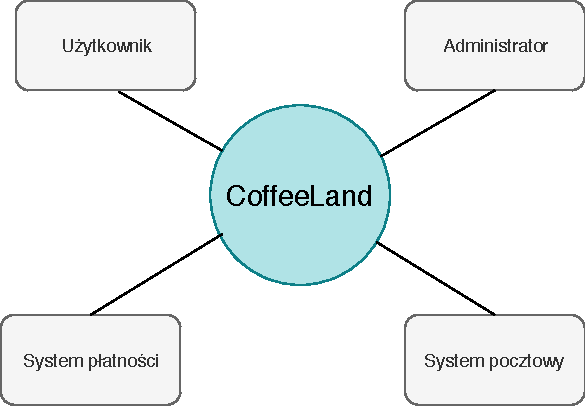
\includegraphics[width=400pt]{kontekstowy.pdf}
	\end{center}
%---------------------------------------	
%---------------------------------------
%---------------------------------------
	
	\chapter{Funkcjonalności}
	
	
%---------------------------------------
\section{Rejstracja}
	\subsection{Opis przypadku użycia}
	\begin{table}[h]
		\def\arraystretch{1.3}
		\begin{tabular}{|>{\columncolor[gray]{0.97}}p{4cm}| p{12cm} |}
			\hline
			\textbf{Aktorzy}		
					& Użytkownik 			\\ \hline
			\textbf{Zakres}    		
					& Sklep internetowy     \\ \hline
			\textbf{Poziom}     	
					& Sytemowowy            \\ \hline
			\textbf{Udziałowcy i cele}	
					& Użytkownik chce stworzyć konto. Sklep chce zebrać dane spełniające zadane warunki.           					\\ \hline
			\textbf{\begin{tabular}[l]{@{}l@{}}Zdarzenie \\ wyzwalające\end{tabular}} 	
					& Użytkownik przechodzi na podstronę ‘Sign in/Register’ 														\\ \hline
			\textbf{Warunki wstępne}	
					& Użytkownik nie jest zalogowany																											\\ \hline
			\textbf{\begin{tabular}[l]{@{}l@{}}Warunki końcowe \\ dla sukcesu\end{tabular}}     
					& Konto użytkownika zostaje utworzone i zapisane w bazie danych. Użytkownik zostaje powiadomiony o sukcesie.  	\\ \hline
			\textbf{\begin{tabular}[l]{@{}l@{}}Warunki końcowe \\ dla niepowodzenia\end{tabular}}   
					& Konto nie zostaje stworzone. Użytkownik zostaje powiadomiony o niepowodzeniu i przyczynach niepowodzenia. 	\\ \hline
		\end{tabular}
	\end{table}
%---------------------------------------
	\colorbox{grey}{Scenariusz główny:}
		\begin{enumerate}
			\item System wyświetla formularz wprowadzania danych rejestracji
			\item Użytkownik wprowadza dane (zdefiniowane w słowniku): imię, nazwisko, email, hasło
			\item System weryfikuje dane
			\item System wyświetla powiadomienie o udanej rejestracji
		\end{enumerate}
%---------------------------------------	
	
	\colorbox{grey}{Scenariusz alternatywny:}
		\begin{enumerate}\addtocounter{enumi}{2}
			\item[]
			\begin{enumerate}
				\item[2.1] Nie wprowadzono wymaganych danych
				\begin{enumerate}
					\item System wyświetla ponownie formularz zaznaczając, które dane powinny zostać poprawione i jakie warunki powinny spełniać zaznaczone dane
					\item Następuje powrót do punktu 2 scenariusza głównego
				\end{enumerate}
			\end{enumerate}
		\end{enumerate}
%---------------------------------------

	\colorbox{grey}{Scenariusz alternatywny:}
	\begin{enumerate}\addtocounter{enumi}{2}
		\item[]
		\begin{enumerate}
			\item[2.2] W bazie danych znajduję się konto dla podanego email’a
			\begin{enumerate}
				\item System wyświetla ponownie formularz zaznaczając email i wyświetla informację o istnieniu konta dla podanego email’a
				\item Następuje powrót do punktu 2 scenariusza głównego
			\end{enumerate}
		\end{enumerate}
	\end{enumerate}


	\subsection{Model przypadku użycia}
	\begin{center}
		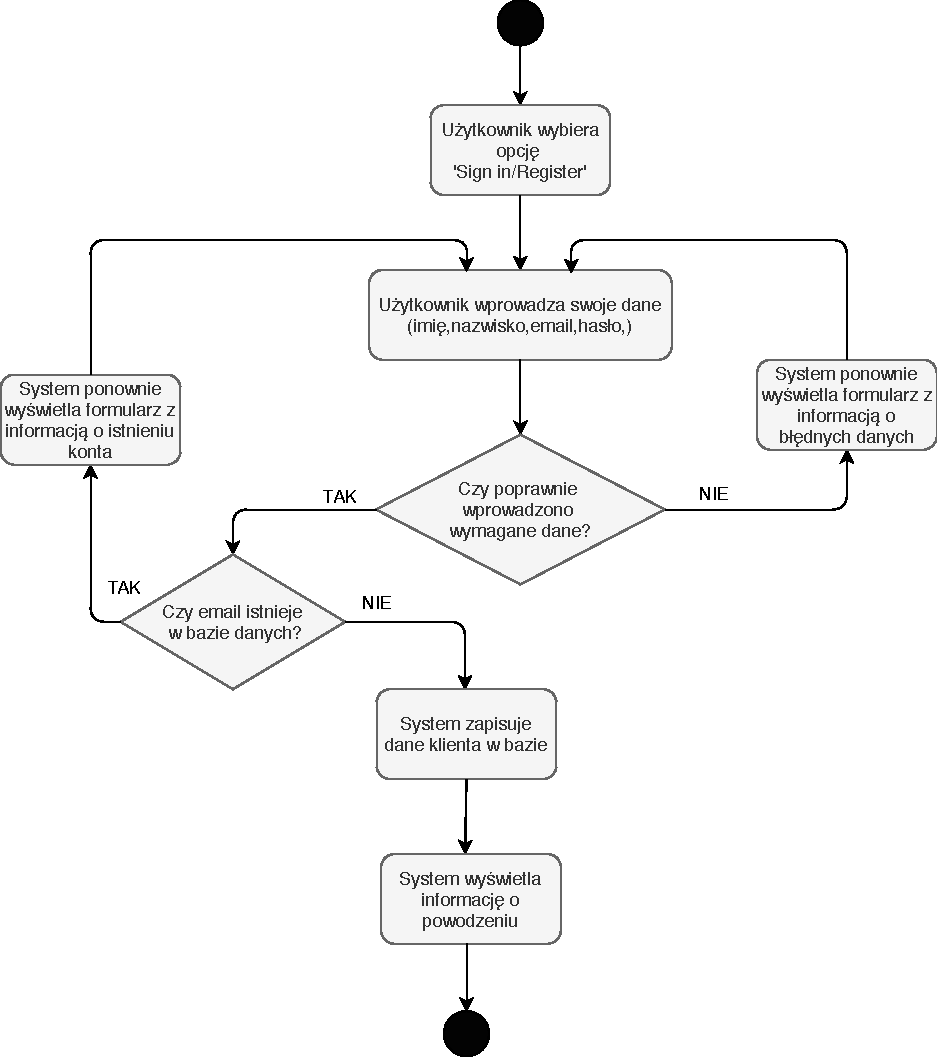
\includegraphics[width=400pt]{rejstracja.pdf}
	\end{center}
	
	\newpage
%---------------------------------------
%---------------------------------------
%---------------------------------------

\section{Logowanie}
	\subsection {Opis przypadku użycia}
	
	\begin{table}[h]
		\def\arraystretch{1.3}
		\begin{tabular}{|>{\columncolor[gray]{0.97}}p{4cm}| p{12cm} |}
			\hline
			\textbf{Aktorzy}		
			& Użytkownik 			\\ \hline
			\textbf{Zakres}    		
			& Sklep internetowy     \\ \hline
			\textbf{Poziom}     	
			& Sytemowowy            \\ \hline
			\textbf{Udziałowcy i cele}	
			& Użytkownik chce się zalogować. Sklep chce zebrać dane spełniające zadane warunki.           					\\ \hline
			\textbf{\begin{tabular}[l]{@{}l@{}}Zdarzenie \\ wyzwalające\end{tabular}} 	
			& Użytkownik przechodzi na podstronę ‘Sign in/Register’ 														\\ \hline
			\textbf{Warunki wstępne}	
			& 
			Użytkownik nie jest zalogowany									\\ \hline
			\textbf{\begin{tabular}[l]{@{}l@{}}Warunki końcowe \\ dla sukcesu\end{tabular}}     
			& Użytkownik zastaje zalogowany. Następuje przekierowanie na podstronę 'Shop'. 	\\ \hline
			\textbf{\begin{tabular}[l]{@{}l@{}}Warunki końcowe \\ dla niepowodzenia\end{tabular}}   
			& Użytkownik nie zostaje zalogowany. Użytkownik zostaje powiadomiony o niepowodzeniu. 	\\ \hline
		\end{tabular}
	\end{table}

\newpage
	%---------------------------------------
	\colorbox{grey}{Scenariusz główny:}
	\begin{enumerate}
		\item System wyświetla formularz wprowadzania danych logowania
		\item Użytkownik wprowadza dane: email, hasło
		\item System weryfikuje czy w bazie danych istnieje konto, które odpowiada wprowadzonym danym
		\item System przekierowuje na podstronę ‘Shop’.
		\item System wyświetla ‘My account’ na pasku nawigacji
		\item System zamienia opcję przekierowania na postronę ‘Sign in/Register’ na opcję wylogowania użytkownika ‘Sign out’
		%\item Użytkownik przechodzi na podstronę ‘My account’
	\end{enumerate}
	%---------------------------------------	
	
	\colorbox{grey}{Scenariusz alternatywny:}
	\begin{enumerate}\addtocounter{enumi}{3}
		\item[]
		\begin{enumerate}
			\item Nie istnieje konto dla wprowadzonych danych
			\begin{enumerate}
				\item System wyświetla informację o niepowodzeniu
				\item Następuje powrót do punktu 2 scenariusza głównego
			\end{enumerate}
		\end{enumerate}
	\end{enumerate}
	%---------------------------------------

	\subsection{Model przypadku użycia}
	\begin{center}
		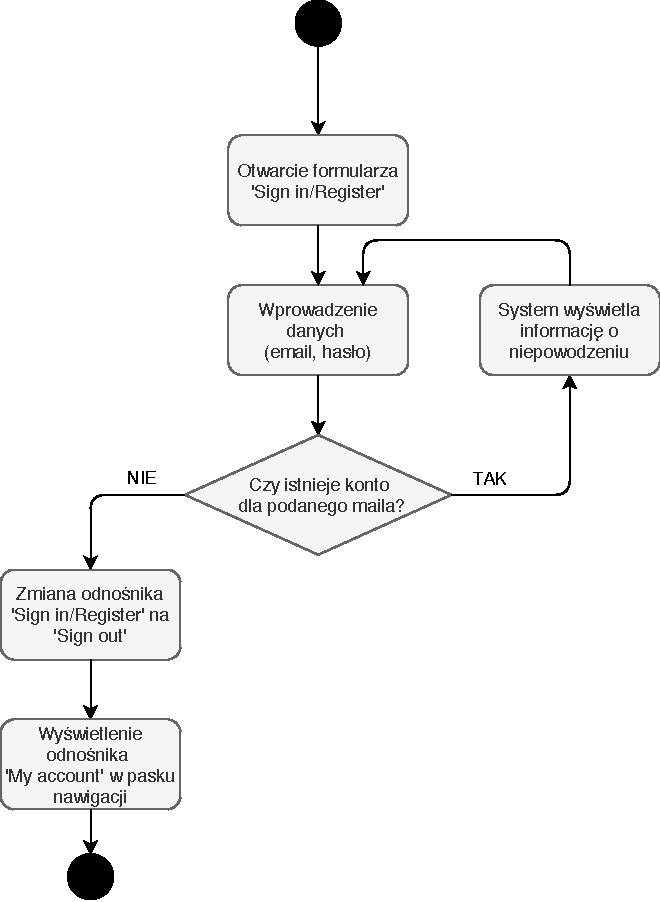
\includegraphics[width=300pt]{logowanie.pdf}
	\end{center}
\newpage


%---------------------------------------		
\section{Wylogowanie}
	\subsection{Opis przypadku użycia}
	
	\begin{table}[h]
		\def\arraystretch{1.3}
		\begin{tabular}{|>{\columncolor[gray]{0.97}}p{4cm}| p{12cm} |}
			\hline
			\textbf{Aktorzy}		
			& Użytkownik 			\\ \hline
			\textbf{Zakres}    		
			& Sklep internetowy     \\ \hline
			\textbf{Poziom}     	
			& Sytemowowy            \\ \hline
			\textbf{Udziałowcy i cele}	
			& Użytkownik chce się wylogować. Sklep chce poprawnie wykonać operację.           					\\ \hline
			\textbf{\begin{tabular}[l]{@{}l@{}}Zdarzenie \\ wyzwalające\end{tabular}} 	
			& Użytkownik przechodzi na podstronę ‘Sign out’ 														\\ \hline
			\textbf{Warunki wstępne}	
			& 
			Użytkownik jest zalogowany									\\ \hline
			\textbf{\begin{tabular}[l]{@{}l@{}}Warunki końcowe \\ dla sukcesu\end{tabular}}     
			& Użytkownik zastaje wylogowany. Następuje przekierowanie na podstronę 'Shop'. 	\\ \hline
		
		\end{tabular}
	\end{table}
	
	%---------------------------------------
	\colorbox{grey}{Scenariusz główny:}
	\begin{enumerate}
		\item Użytkownik wybiera opcję 'Sign out'
		\item System usuwa odnośnik 'My account' z paska nawigacji
		\item System zamienia opcję przekierowania na podstronę ‘Sign out’ na opcję logowania ‘Sign in/Register’
		\item System przekierowuje na podstronę ‘Shop’.
	\end{enumerate}
	%---------------------------------------	
	
	\subsection{Model przypadku użycia}
	\begin{center}
		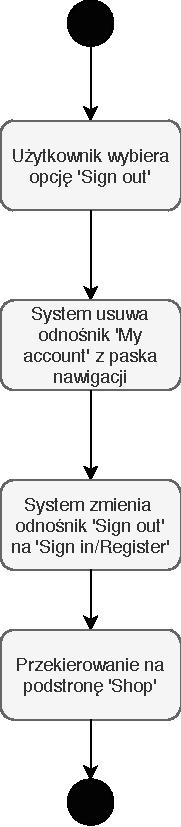
\includegraphics[width=120pt]{wylogowanie.pdf}
	\end{center}
	\newpage
%---------------------------------------
		
	\section{Zmiana zawartości koszyka}
		\subsection{Dodawanie produktów do koszyka z poziomu podstrony produktu}
		\subsubsection{Opis przypadku użycia}
		\begin{table}[h]
			\def\arraystretch{1.3}
			\begin{tabular}{|>{\columncolor[gray]{0.97}}p{4cm}| p{12cm} |}
				\hline
				\textbf{Aktorzy}		
				& Użytkownik 			\\ \hline
				\textbf{Zakres}    		
				& Sklep internetowy     \\ \hline
				\textbf{Poziom}     	
				& Sytemowowy            \\ \hline
				\textbf{Udziałowcy i cele}	
				& Użytkownik chce dodać produkty do koszyka. Sklep chce zebrać i zapisać informacje o zawartości koszyka.           					\\ \hline
				\textbf{\begin{tabular}[l]{@{}l@{}}Zdarzenie \\ wyzwalające\end{tabular}} 	
				& Użytkownik przechodzi na podstronę produktu. 														\\ \hline
				\textbf{Warunki wstępne}	
				& brak 																											\\ \hline
				\textbf{\begin{tabular}[l]{@{}l@{}}Warunki końcowe \\ dla sukcesu\end{tabular}}     
				& Dodanie produktu do koszyka.	\\ \hline
			\end{tabular}
		\end{table}
		
		%---------------------------------------
		\colorbox{grey}{Scenariusz główny:}
		\begin{enumerate}
			\item System wyświetla podstronę produktu
			\item Użytkownik wprowadza ilość produktów
			\item System weryfikuje dane 
			\item Użytkownik wybiera opcję 'Add to Cart'
			\item System zmienia stan koszyka
			\item System wyświetla informację o powodzeniu
		\end{enumerate}
		%---------------------------------------	
	
	
	\newpage
		%---------------------------------------
	\subsubsection{Model przypadku użycia}
	\begin{center}
		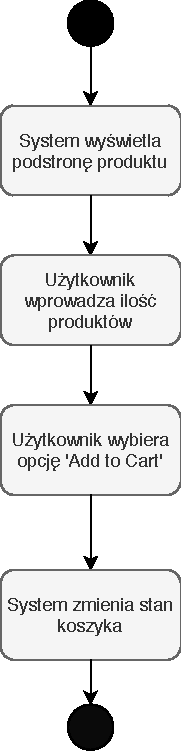
\includegraphics[width=120pt]{koszyk1.pdf}
	\end{center}
		
	%-------------------------------------------------	
		
	\subsection{Zmiana zawartości koszyka z poziomu podstrony koszyka}
	\subsubsection{Opis przypadku użycia}
	\begin{table}[h]
		\def\arraystretch{1.3}
		\begin{tabular}{|>{\columncolor[gray]{0.97}}p{4cm}| p{12cm} |}
			\hline
			\textbf{Aktorzy}		
			& Użytkownik 			\\ \hline
			\textbf{Zakres}    		
			& Sklep internetowy     \\ \hline
			\textbf{Poziom}     	
			& Sytemowowy            \\ \hline
			\textbf{Udziałowcy i cele}	
			& Użytkownik chce zmienić zawartość koszyka. Sklep chce zaktualizować informacje o zawartości koszyka.           					\\ \hline
			\textbf{\begin{tabular}[l]{@{}l@{}}Zdarzenie \\ wyzwalające\end{tabular}} 	
			& Użytkownik przechodzi na podstronę koszyka. 														\\ \hline
			\textbf{Warunki wstępne}	
			& brak 																											\\ \hline
			\textbf{\begin{tabular}[l]{@{}l@{}}Warunki końcowe \\ dla sukcesu\end{tabular}}     
			& Aktualizacja stanu koszyka.	\\ \hline
		\end{tabular}
	\end{table}
	
	%---------------------------------------
	\colorbox{grey}{Scenariusz główny:}
	\begin{enumerate}
		\item System wyświetla podstronę koszyka
		\item Użytkownik zmienia ilość produktów
		\item System weryfikuje dane 
		\item System aktualizuje stan koszyka
	\end{enumerate}
	%---------------------------------------	

\newpage

\subsubsection{Model przypadku użycia}
\begin{center}
	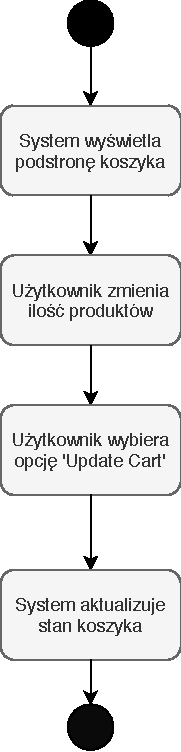
\includegraphics[width=120pt]{koszyk2.pdf}
\end{center}
	%---------------------------------------
	
%---------------------------------------			
	\section{Zakup produktu}
	
	\subsection{Opis przypadku użycia}
	\begin{table}[h]
		\def\arraystretch{1.3}
		\begin{tabular}{|>{\columncolor[gray]{0.97}}p{4cm}| p{12cm} |}
			\hline
			\textbf{Aktorzy}		
			& Użytkownik 			\\ \hline
			\textbf{Zakres}    		
			& Sklep internetowy     \\ \hline
			\textbf{Poziom}     	
			& Sytemowowy            \\ \hline
			\textbf{Udziałowcy i cele}	
			& Użytkownik dokonuje zakupu towarów. Sklep przekierowuje go do procedury płatności.     	\\ \hline
			\textbf{\begin{tabular}[l]{@{}l@{}}Zdarzenie \\ wyzwalające\end{tabular}} 	
			& Użytkownik klika 'Buy' na podstronie koszyka. 	\\ \hline
			\textbf{Warunki wstępne}	
			& Użytkownik jest zalogowany 																											\\ \hline
			\textbf{\begin{tabular}[l]{@{}l@{}}Warunki końcowe \\ dla sukcesu\end{tabular}}     
			& Nastąpi przekierowanie do procedury płatności.	\\ \hline
			\textbf{\begin{tabular}[l]{@{}l@{}}Warunki końcowe \\ dla niepowodzenia\end{tabular}}   
			& Użytkownik zostanie powiadomiony o niepowodzeniu. \\ \hline
		\end{tabular}
	\end{table}
	
	%---------------------------------------
	\colorbox{grey}{Scenariusz główny:}
	\begin{enumerate}
		\item Użytkownik przechodzi na podstronę Koszyka.
		\item Użytkownik klika 'Buy'.
		\item System sprawdza, czy użytkownik jest zalogowany.
		\item System przekierowywuje użytkownika na stronę 'Checkout Details'.
		\item Użytkownik wykonuje jeden ze scenariuszy odnoszących się do scenariusza CHECKOUT DETAILS (WYSYŁKA).
		\item System przekazuje dane z koszyka do systemu płatniczego, i przekierowywuje na formularz wymagający uwierzytelnienia.
	\end{enumerate}
	%---------------------------------------	
	
	\colorbox{grey}{Scenariusz alternatywny:}
	\begin{enumerate}\addtocounter{enumi}{6}
		\item[]
		\begin{enumerate}
			\item[3.1] Użytkownik nie jest zalogowany.
			\begin{enumerate}
				\item System przekierowywuje użytkownika do postrony z logowaniem.
				\item Użytkownik realizuje jeden ze scenariuszy ze scenariusza LOGOWANIE.
				\item Następuje powrót do punktu 1. scenariusza głównego.
			\end{enumerate}
		\end{enumerate}
	\end{enumerate}

	\subsection{Model przypadku użycia}
	\begin{center}
		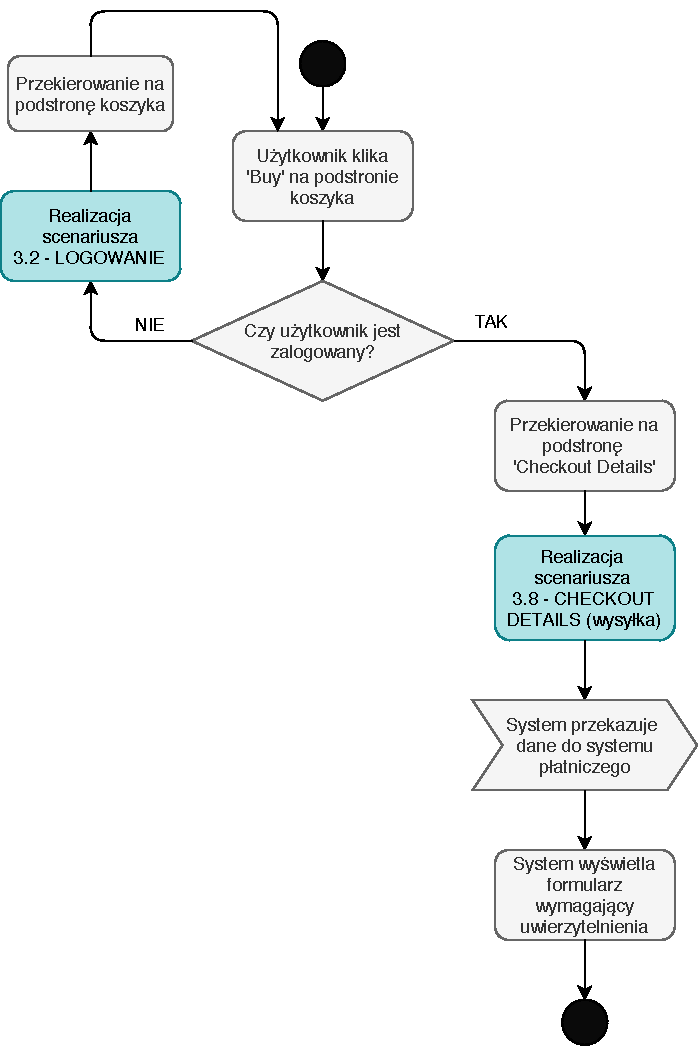
\includegraphics[width=350pt]{zakup.pdf}
	\end{center}
%-------------------------------------------------

	
	\section{Edycja danych osobowych}
	\subsection{Opis przypadku użycia}
	\begin{table}[h]
		\def\arraystretch{1.3}
		\begin{tabular}{|>{\columncolor[gray]{0.97}}p{4cm}| p{12cm} |}
			\hline
			\textbf{Aktorzy}		
			& Użytkownik 			\\ \hline
			\textbf{Zakres}    		
			& Sklep internetowy     \\ \hline
			\textbf{Poziom}     	
			& Sytemowowy            \\ \hline
			\textbf{Udziałowcy i cele}	
			& Użytkownik zmienia swoje dane osobowe, oraz adres e-mail. Sklep zapisuje nowopodane dane.          					\\ \hline
			\textbf{\begin{tabular}[l]{@{}l@{}}Zdarzenie \\ wyzwalające\end{tabular}} 	
			& Wybranie opcji 'Personal Informations' w podstronie widocznej po zalogowaniu użytkownika. 				\\ \hline
			\textbf{Warunki wstępne}	
			& Użytkownik jest zalogowany. 																											\\ \hline
			\textbf{\begin{tabular}[l]{@{}l@{}}Warunki końcowe \\ dla sukcesu\end{tabular}}     
			& System zapisuje nowe dane uzytkownika. 	\\ \hline
			\textbf{\begin{tabular}[l]{@{}l@{}}Warunki końcowe \\ dla niepowodzenia\end{tabular}}   
			& System wysyła komunikat o błędzie i powraca do formularza z danymi osobowymi. 	\\ \hline
		\end{tabular}	
	\end{table}
	
	%---------------------------------------
	\colorbox{grey}{Scenariusz główny:}
	\begin{enumerate}
		\item Użytkownik wybiera opcję 'Personal Information'.
		\item System wyświetla na stronie widok formularza.
		\item Użytkownik wypełnia formularz.
		\item Użytkownik klika 'OK'.
		\item System weryfikuje dane.
		\item System wysyła komunikat o zapisie danych.
	\end{enumerate}
	%---------------------------------------	
	
	\colorbox{grey}{Scenariusz alternatywny:}
	\begin{enumerate}\addtocounter{enumi}{5}
		\item[]
		\begin{enumerate}
			\item System odrzuca zmiany.
			\begin{enumerate}
				\item System wyświetla komunikat o niepoprawności danych.
				\item Następuje powrót do punktu 3. scenariusza głównego.
			\end{enumerate}
		\end{enumerate}
	\end{enumerate}

	\subsection{Model przypadku użycia}
%-----------------------------------------------
	\begin{center}
		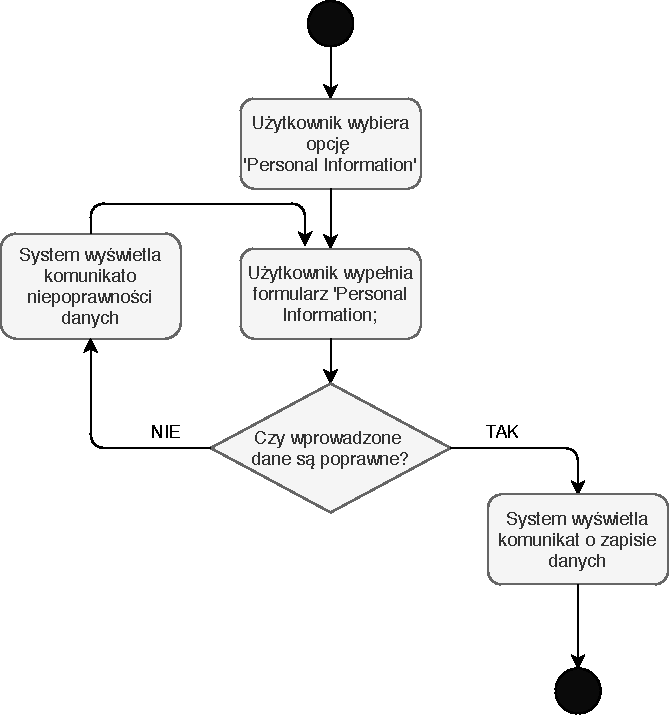
\includegraphics[width=400pt]{edycja.pdf}
	\end{center}
	\newpage
%------------------------------------------
	%----------------------------------------
	
	\section{Reklamacja}
		\subsection{Opis przypadku użycia}
		\begin{table}[h]
			\def\arraystretch{1.3}
			\begin{tabular}{|>{\columncolor[gray]{0.97}}p{4cm}| p{12cm} |}
				\hline
				\textbf{Aktorzy}		
				& Użytkownik 			\\ \hline
				\textbf{Zakres}    		
				& Sklep internetowy     \\ \hline
				\textbf{Poziom}     	
				& Sytemowowy            \\ \hline
				\textbf{Udziałowcy i cele}	
				& Użytkownik chce dokonać reklamacji. 
				Sklep chce zebrać dane spełniające zadane warunki.            					\\ \hline
				\textbf{\begin{tabular}[l]{@{}l@{}}Zdarzenie \\ wyzwalające\end{tabular}} 	
				&Użytkownik przechodzi na podstronę ‘My account’								\\ \hline
				\textbf{Warunki wstępne}	
				& Użytkownik jest zalogowany. 																											\\ \hline
				\textbf{\begin{tabular}[l]{@{}l@{}}Warunki końcowe \\ dla sukcesu\end{tabular}}     
				& Reklamacja zostaje zapisana w bazie danych. 
				Użytkownik zostaje powiadomiony o sukcesie	\\ \hline
				\textbf{\begin{tabular}[l]{@{}l@{}}Warunki końcowe \\ dla niepowodzenia\end{tabular}}   
				& Użytkownik zostaje powiadomiony o niepowodzeniu i przyczynach niepowodzenia.
					\\ \hline
			\end{tabular}
			
			
		\end{table}
		
		%---------------------------------------
		\colorbox{grey}{Scenariusz główny:}
		\begin{enumerate}
			\item Użytkownik przechodzi na zakładkę ‘Orders’.
			\item Użytkownik wybiera opcję ‘Complain’
			\item System otwiera podstronę ‘Complain’
			\item Użytkownik wprowadza dane w polu ‘Letter of complain’
			\item System weryfikuje dane (czy wprowadzono minimum 10 znaków)
			\item System wyświetla powiadomienie o udanej reklamacji
		\end{enumerate}
		%---------------------------------------	
	
		\colorbox{grey}{Scenariusz alternatywny:}
		\begin{enumerate}\addtocounter{enumi}{2}
			\item[]
			\begin{enumerate}
				\item[5.1] Nie wprowadzono wymaganych danych
				\begin{enumerate}
					\item System wyświetla ponownie formularz zaznaczając ile znaków należy wprowadzić
					\item Następuje powrót do punktu 4 scenariusza głównego
				\end{enumerate}
			\end{enumerate}
		\end{enumerate}
		
		\newpage
		\subsection{Model przypadku użycia}
			\begin{center}
			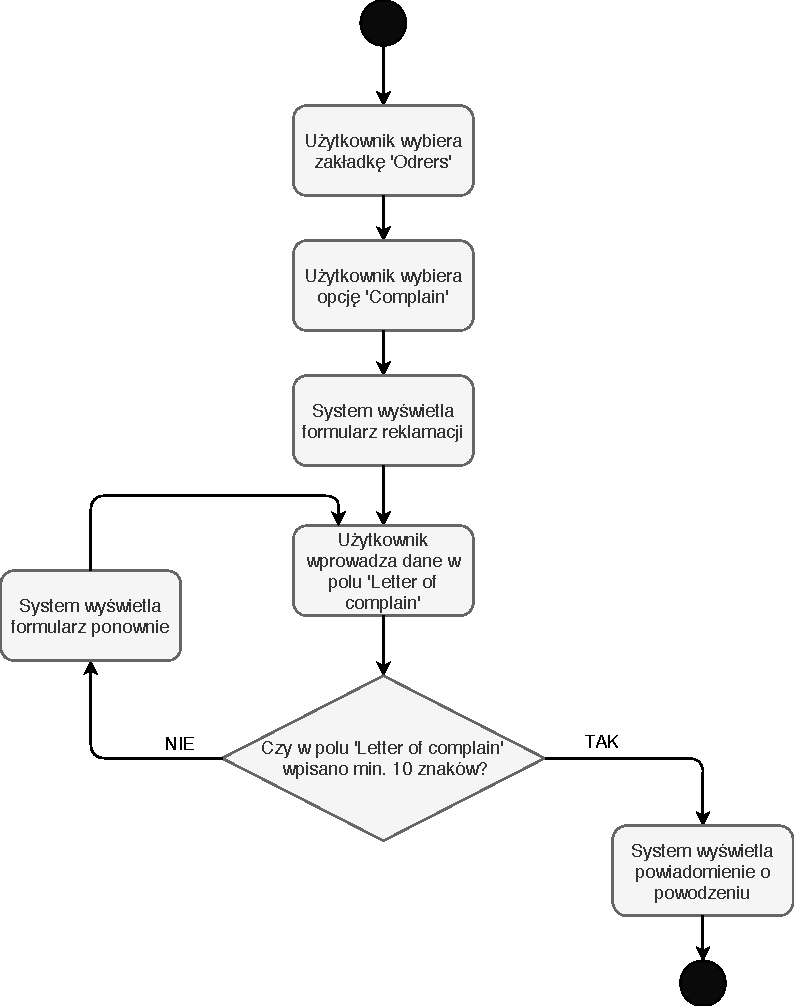
\includegraphics[width=400pt]{reklamacja.pdf}
		\end{center}
		\newpage
	%----------------------------------------
	\section{Checkout details (wysyłka)}
	
	\subsection{Opis przypadku użycia}
	\begin{table}[h]
		\def\arraystretch{1.3}
		\begin{tabular}{|>{\columncolor[gray]{0.97}}p{4cm}| p{12cm} |}
			\hline
			\textbf{Aktorzy}		
			& Użytkownik 			\\ \hline
			\textbf{Zakres}    		
			& Sklep internetowy     \\ \hline
			\textbf{Poziom}     	
			& Sytemowowy            \\ \hline
			\textbf{Udziałowcy i cele}	
			& Użytkownik określa adres wysyłki. System pobiera określony przez użytkownika adres jako dane do wysyłki.            					\\ \hline
			\textbf{\begin{tabular}[l]{@{}l@{}}Zdarzenie \\ wyzwalające\end{tabular}} 	
			&Użytkownik klika 'Next' na podstronie z danymi adresowymi.									\\ \hline
			\textbf{Warunki wstępne}	
			& Użytkownik jest zalogowany. 																											\\ \hline
			\textbf{\begin{tabular}[l]{@{}l@{}}Warunki końcowe \\ dla sukcesu\end{tabular}}     
			& Podany przez użytkownika adres zostanie podany jako
			informacja dla sklepu. 	\\ \hline
			\textbf{\begin{tabular}[l]{@{}l@{}}Warunki końcowe \\ dla niepowodzenia\end{tabular}}   
			& Nastąpi przekierowanie do podstrony z wyborem adresu wysyłki. 	\\ \hline
		\end{tabular}
		
		
	\end{table}
	
	%---------------------------------------
	\colorbox{grey}{Scenariusz główny:}
	\begin{enumerate}
		\item System przekierowywuje zalogowanego użytkownika na podstronę z wyborem adresu.
		\item Użytkownik klika na przycisk rozwijający listę zapisanych adresów.
		\item System wyświetla tę listę, zaznaczając w widoczny sposób adres domyślny.
		\item Użytkownik klika na jeden z innych adresów na liście.
		\item System zaznacza w widoczny sposób wybrany adres i ustawia go jako domyślny.
		\item Użytkownik klika 'Next'
		\item System przekazuje zaznaczony adres jako dane do wysyłki.
	\end{enumerate}
	%---------------------------------------	
	\newpage
	\colorbox{grey}{Scenariusz alternatywny:}
	\begin{enumerate}\addtocounter{enumi}{2}
		\item[]
		\begin{enumerate}
			\item[2.1] Użytkownik klika 'Next'.
			\begin{enumerate}
				\item Następuje przekierownie do punktu 7. scenariusza głównego.
			\end{enumerate}
		\end{enumerate}
	\end{enumerate}

	\colorbox{grey}{Scenariusz alternatywny:}
	\begin{enumerate}\addtocounter{enumi}{2}
		\item[]
		\begin{enumerate}
			\item[2.2] Użytkownik klika 'Add new address'.
				\begin{enumerate}
					\item System rozwija widok z formularzem do danych adresowych.
					\item Użytkownik wypełnia pola formularza.
					\item Użytkownik klika 'Save'.
					\item System sprawdza poprawność danych.
					\item System odznacza adres domyślny z listy, a zaznacza ten podany w formularzu.
					\item Następuje powrót do punktu 6. scenariusza głównego.	
				\end{enumerate}
		\end{enumerate}
	\end{enumerate}
	%---------------------------------------
	
	\colorbox{grey}{Scenariusz alternatywny:}
	\begin{enumerate}\addtocounter{enumi}{2}
		\item[]
		\begin{enumerate}
			\item[2.2.iii.1.] Użytkownik klika 'Add to my Address Book'.
			\begin{enumerate}
				\item System otrzymuje informację o tym, by w punkcie 2.2.iii scenariusza alternatywnego dodać podany adres do bazy danych jako adres klienta.
				\item Nastepuje powrót do punktu 2.2.iii
			\end{enumerate}
		\end{enumerate}
	\end{enumerate}
	
	%---------------------------------------	
	\colorbox{grey}{Scenariusz alternatywny:}
	\begin{enumerate}\addtocounter{enumi}{2}
		\item[]
		\begin{enumerate}
			\item[2.2.iv.1] System odrzuca dane.
			\begin{enumerate}
				\item Następuje powrót do punktu 2.2.iii scenariusza alternatywnego.
			\end{enumerate}
		\end{enumerate}
	\end{enumerate}
	
	\newpage
	
	\subsection{Model przypadku użycia}
	\begin{center}
		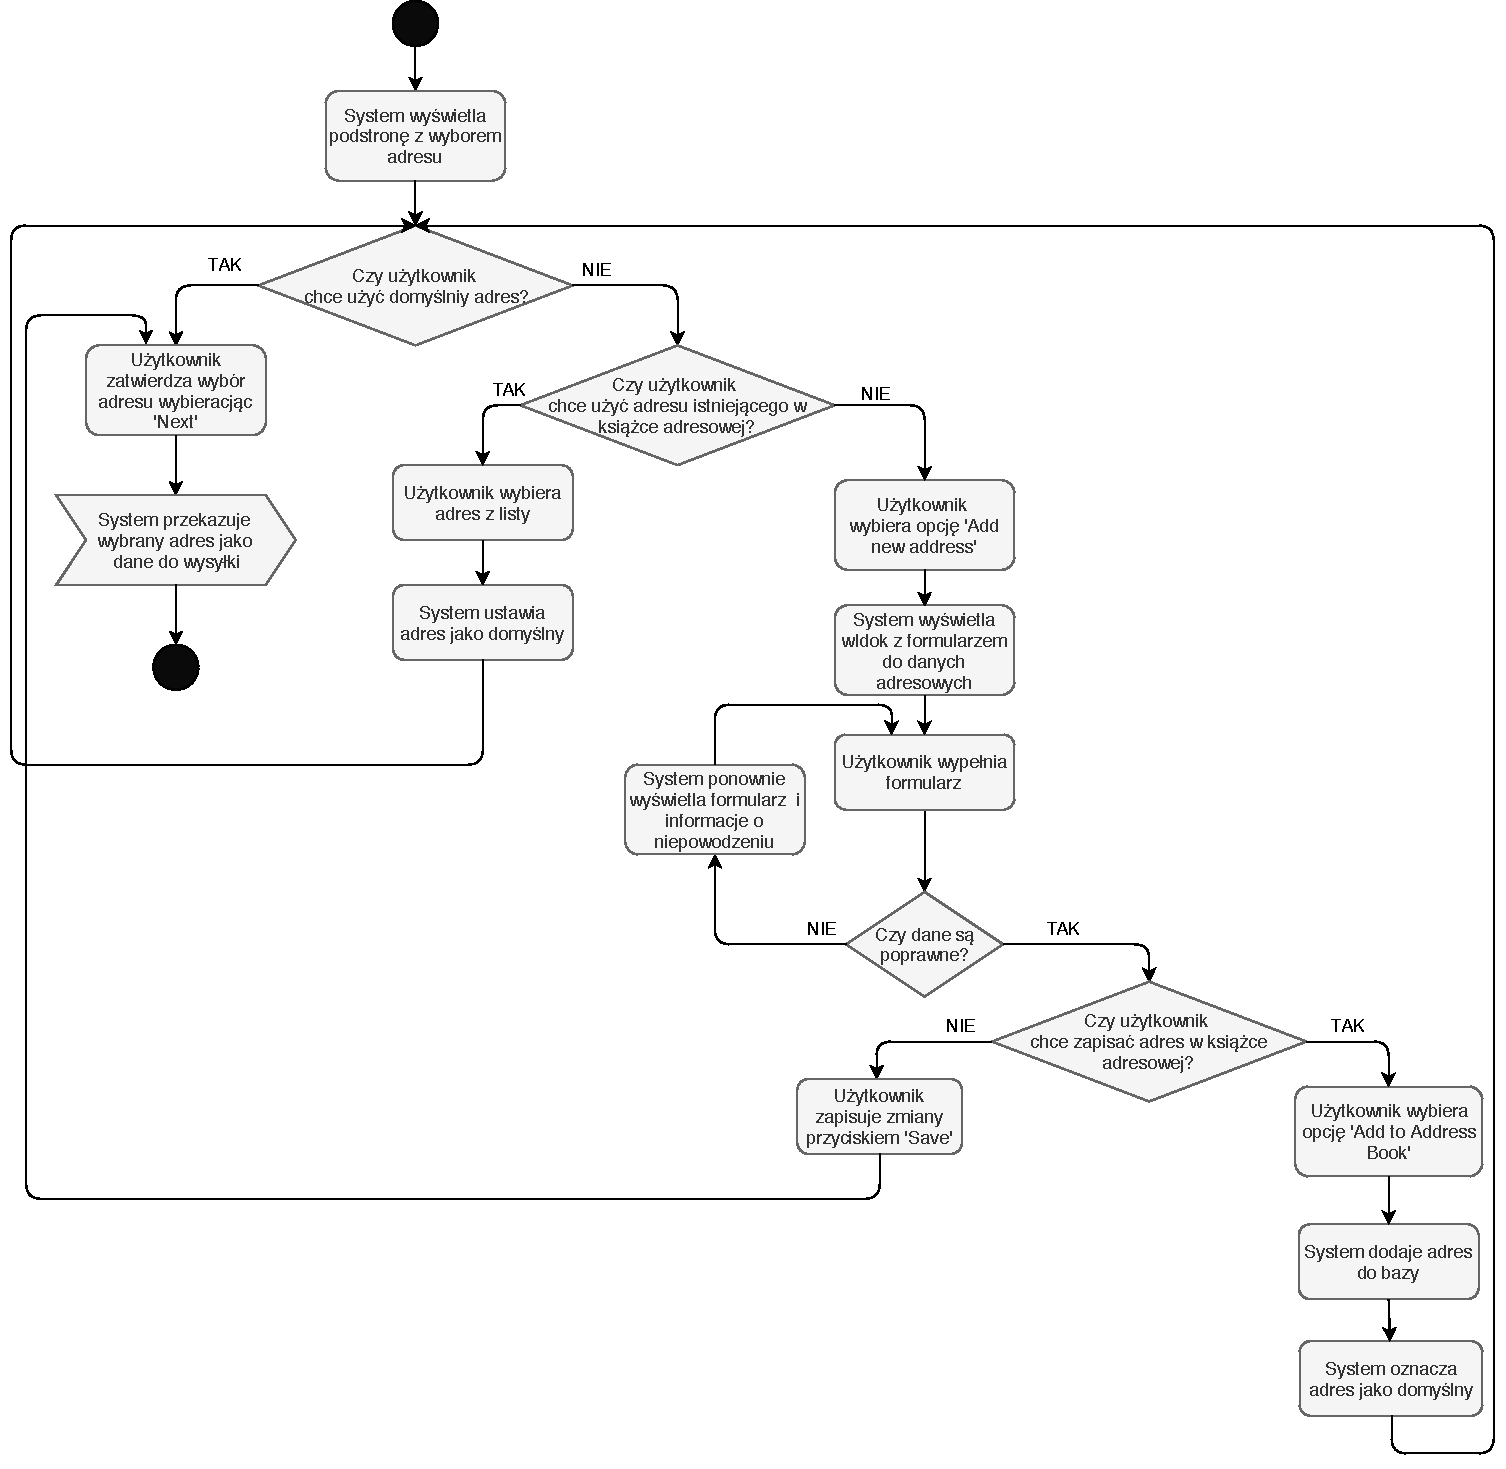
\includegraphics[width=450pt]{wysylka.pdf}
	\end{center}
	\newpage
	
	%----------------------------------------
	
	\section{Checkout details (ustawienia)}
	
	\subsection{Opis przypadku użycia}
	\begin{table}[h]
		\def\arraystretch{1.3}
		\begin{tabular}{|>{\columncolor[gray]{0.97}}p{4cm}| p{12cm} |}
			\hline
			\textbf{Aktorzy}		
			& Użytkownik 			\\ \hline
			\textbf{Zakres}    		
			& Sklep internetowy     \\ \hline
			\textbf{Poziom}     	
			& Sytemowowy            \\ \hline
			\textbf{Udziałowcy i cele}	
			& Użytkownik dodaje/edytuje/usuwa adres wysyłki do swojej listy adresów.
			System modyfikuje listę adresów według polecenia użytkownika.           					\\ \hline
			\textbf{\begin{tabular}[l]{@{}l@{}}Zdarzenie \\ wyzwalające\end{tabular}} 	
			& Użytkownik klika 'My Addresses' na podstronie widoczej bezpośrednio
			po zalogowaniu.								\\ \hline
			\textbf{Warunki wstępne}	
			& Użytkownik jest zalogowany. 																											\\ \hline
			\textbf{\begin{tabular}[l]{@{}l@{}}Warunki końcowe \\ dla sukcesu\end{tabular}}     
			& System wykona żądaną operację. 	\\ \hline
			\textbf{\begin{tabular}[l]{@{}l@{}}Warunki końcowe \\ dla niepowodzenia\end{tabular}}   
			& Nastąpi powrót do widoku z listą adresów, i nie zajdą żadne zmiany. \\ \hline
		\end{tabular}
		
		
	\end{table}
	
	%---------------------------------------
	\colorbox{grey}{Scenariusz główny:}
	\begin{enumerate}
		\item Użytkownik klika 'My Addresses'.
		\item System przekierowywuje go na podstronę z wyborem adresu.
		\item Użytkownik klika na przycisk rozwijający listę zapisanych adresów.
		\item System wyświetla tę listę, zaznaczając w widoczny sposób adres domyślny.
		\item System wyświetla przy elemencie przyciski 'Edit' i 'Delete'.
		\item Użytkownik klika 'Edit'.
		\item System rozwija widok z formularzem do danych adresowych.
		\item System wypełnia pola wartościami tworzącymi adres.
		\item Użytkownik edytuje pola formularza.
		\item Użytkownik klika 'Save'.
		\item System weryfikuje poprawność danych.
		\item System zapisuje zmiany.
	\end{enumerate}
	%---------------------------------------
		
	\colorbox{grey}{Scenariusz alternatywny:}
	\begin{enumerate}\addtocounter{enumi}{2}
		\item[]
		\begin{enumerate}
			\item[3.1] Użytkownik klika 'Add new Address'.
			\begin{enumerate}
				\item System rozwija widok z formularzem do danych adresowych.
				\item Następuje powrót do punktu 10. scenariusza głównego.
			\end{enumerate}
		\end{enumerate}
	\end{enumerate}
	
	\colorbox{grey}{Scenariusz alternatywny:}
	\begin{enumerate}\addtocounter{enumi}{6}
		\item[]
		\begin{enumerate}
			\item[6.1] Użytkownik klika 'Delete'.
			\begin{enumerate}
				\item System usuwa element z listy.
				\item Następuje powrót do punktu 12 scenariusza głównego
			\end{enumerate}
		\end{enumerate}
	\end{enumerate}

	\colorbox{grey}{Scenariusz alternatywny:}
	\begin{enumerate}\addtocounter{enumi}{6}
		\item[]
		\begin{enumerate}
			\item[11.1] Wprowadzone dane są błędne.
			\begin{enumerate}
				\item System ponownie wyświetla formularz z informacją o niepowodzeniu.
				\item Następuje powrót do punktu 9 scenariusza głównego.
			\end{enumerate}
		\end{enumerate}
	\end{enumerate}
	%---------------------------------------
	
	\subsection{Model przypadku użycia}
	\begin{center}
		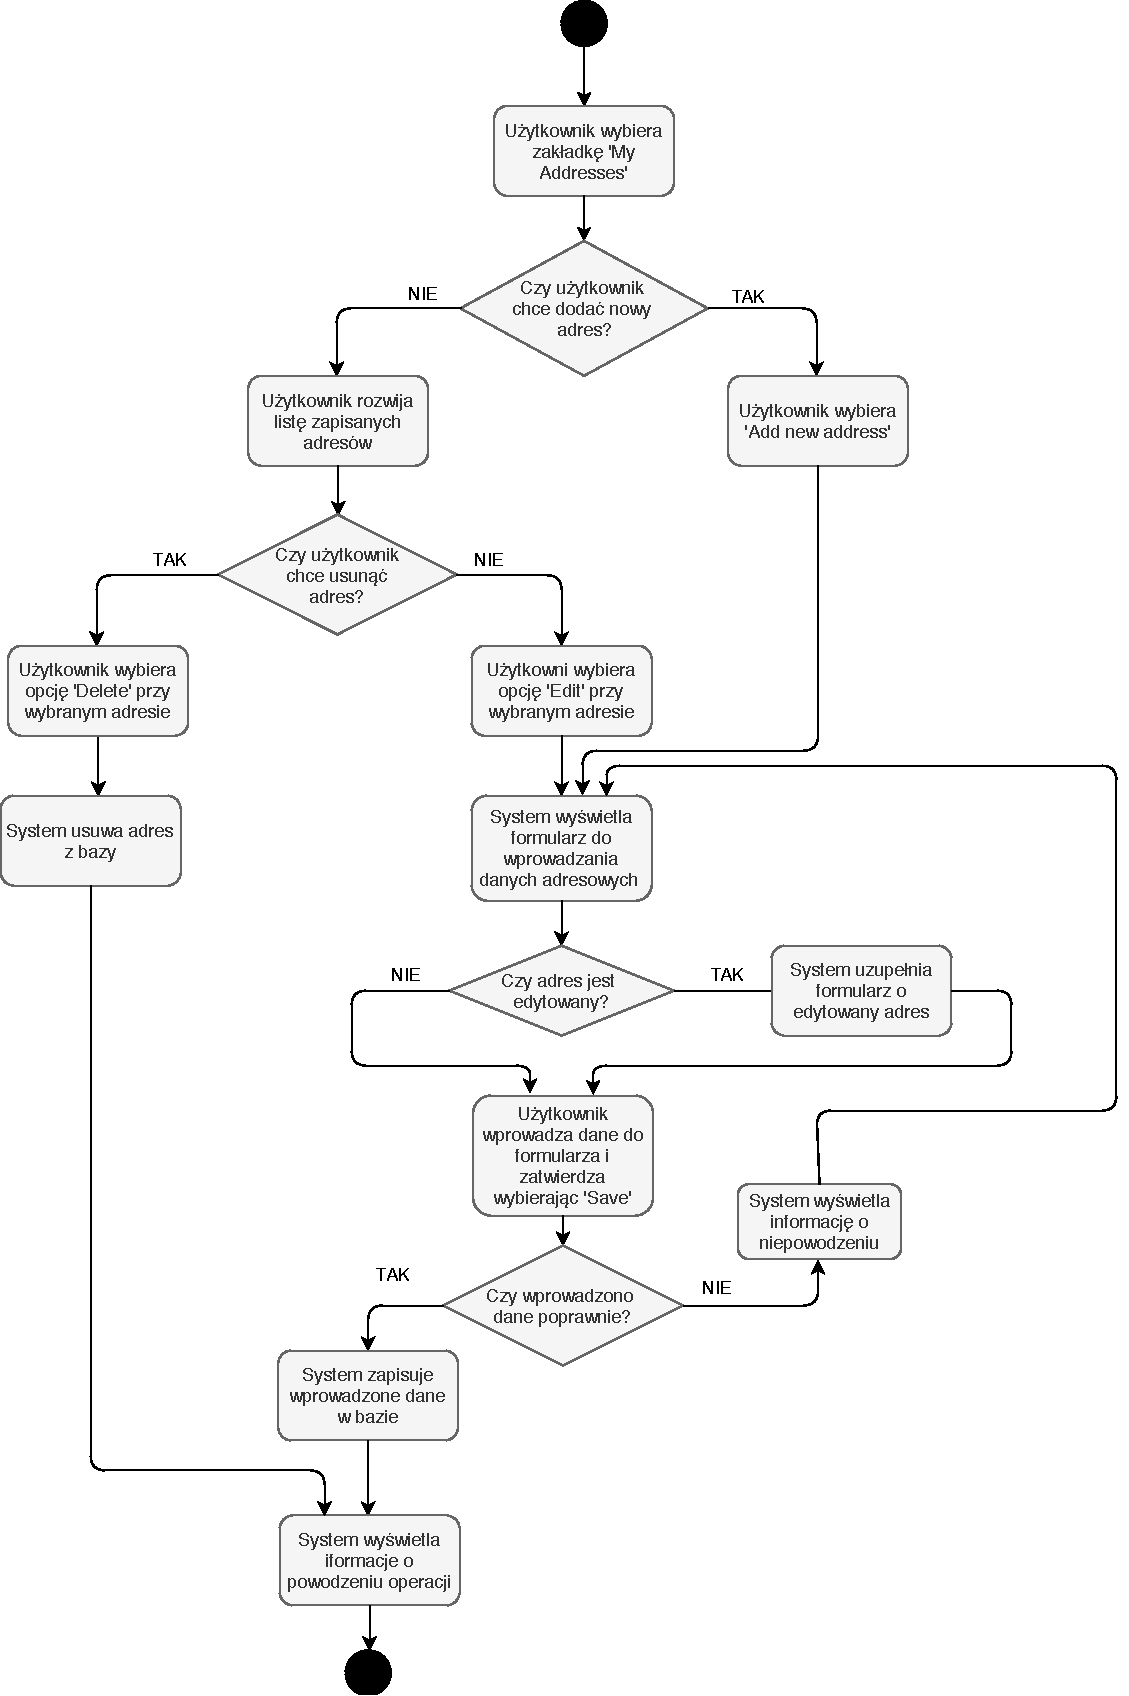
\includegraphics[width=350pt]{ustawienia.pdf}
	\end{center}
	\newpage
	
	%---------------------------------------
	
	
	%---------------------------------------
	
	\section{Filtrowanie produktów}
		\subsection{Opis przypadku użycia}
	\begin{table}[h]
		\def\arraystretch{1.3}
		\begin{tabular}{|>{\columncolor[gray]{0.97}}p{4cm}| p{12cm} |}
			\hline
			\textbf{Aktorzy}		
			& Użytkownik 			\\ \hline
			\textbf{Zakres}    		
			& Sklep internetowy     \\ \hline
			\textbf{Poziom}     	
			& Sytemowowy            \\ \hline
			\textbf{Udziałowcy i cele}	
			& Użytkownik zaznacza typ/cenę szukanego produktu. Sklep redukuje/rozszerza listę produktów o te spełniające zadane warunki.           		\\ \hline
			\textbf{\begin{tabular}[l]{@{}l@{}}Zdarzenie \\ wyzwalające\end{tabular}} 	
			& Zaznaczenie/odznaczenie opcji. 			\\ \hline
			\textbf{Warunki wstępne}	
			& brak 																											\\ \hline
			\textbf{\begin{tabular}[l]{@{}l@{}}Warunki końcowe \\ dla sukcesu\end{tabular}}     
			& System wyświetla produkty spełniające określone kryterium. 	\\ \hline
		\end{tabular}
	\end{table}
	
	%---------------------------------------
	\colorbox{grey}{Scenariusz główny:}
	\begin{enumerate}
		\item Klient wybiera kategorię filtracji.
		\item System wyświetla listę produktów spełniających kryteria
	\end{enumerate}
	%---------------------------------------	
	
	\colorbox{grey}{Scenariusz alternatywny:}
	\begin{enumerate}\addtocounter{enumi}{1}
		\item[]
		\begin{enumerate}
			\item Klient odznacza opcję.
			\begin{enumerate}
				\item System wyświetla listę, rozszerzając ją o produkty spełniające kryteria.
			\end{enumerate}
		\end{enumerate}
	\end{enumerate}
	%---------------------------------------
	
	
	\colorbox{grey}{Scenariusz alternatywny:}
	\begin{enumerate}\addtocounter{enumi}{2}
		\item[]
		\begin{enumerate}
			\item System wyświetla informację, że nie ma produktów spełniających podane kryteria.
		\end{enumerate}
	\end{enumerate}

	\subsection{Model przypadku użycia}
	\begin{center}
		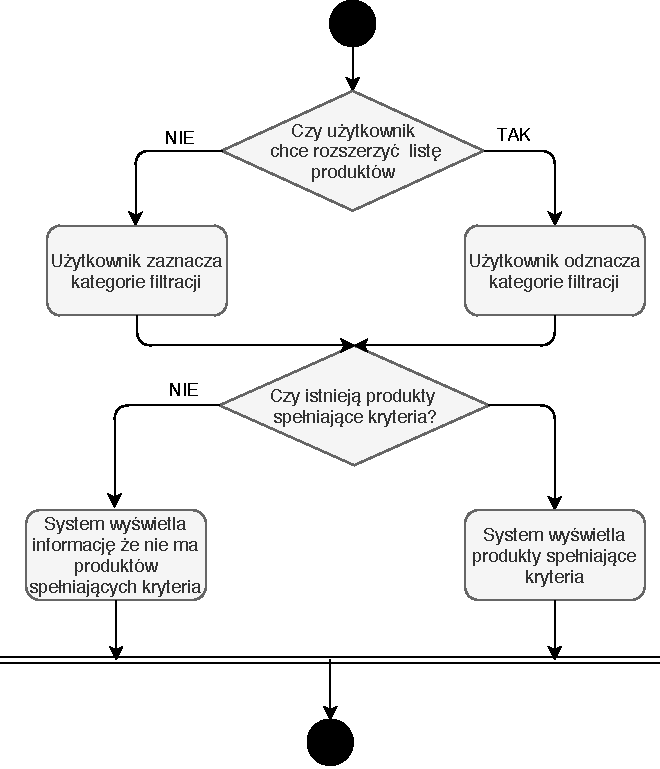
\includegraphics[width=350pt]{filtracja.pdf}
	\end{center}
	\newpage
%-----------------------------------------------------

		\section{Newsletter}
	\subsection{Opis przypadku użycia}
	\begin{table}[h]
		\def\arraystretch{1.3}
		\begin{tabular}{|>{\columncolor[gray]{0.97}}p{4cm}| p{12cm} |}
			\hline
			\textbf{Aktorzy}		
			& Użytkownik 			\\ \hline
			\textbf{Zakres}    		
			& Sklep internetowy     \\ \hline
			\textbf{Poziom}     	
			& Sytemowowy            \\ \hline
			\textbf{Udziałowcy i cele}	
			& Użytkownik chce zapisać się/wypisać z newsletter’a. 
			Sklep chce zebrać informacje o zapisie do newsletter’a	          		\\ \hline
			\textbf{\begin{tabular}[l]{@{}l@{}}Zdarzenie \\ wyzwalające\end{tabular}} 	
			& Użytkownik przechodzi na podstronę ‘My account’ 			\\ \hline
			\textbf{Warunki wstępne}	
			& Użytkownik jest zalogowany 																											\\ \hline
			\textbf{\begin{tabular}[l]{@{}l@{}}Warunki końcowe \\ dla sukcesu\end{tabular}}     
			& Deklaracja dotycząca newsletter’ zostaje zapisana w bazie danych 	\\ \hline
		\end{tabular}
	\end{table}
	
	%---------------------------------------
	\colorbox{grey}{Scenariusz główny:}
	\begin{enumerate}
		\item Użytkownik przechodzi na zakładkę ‘Newsletter’
		\item Użytkownik wybiera opcję zapisu do newsletter’a / rezygnacji z newsletter’a
		\item System aktualizuje informacje na stronie i w bazie danych
	\end{enumerate}
	%---------------------------------------	

	\subsection{Model przypadku użycia}
	\begin{center}
		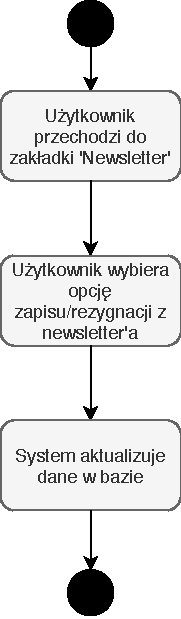
\includegraphics[width=150pt]{newsletter.pdf}
	\end{center}
	\newpage
	
%---------------------------------------	

	\renewcommand{\thesection}{\thechapter.\arabic{section}}		
	
	\chapter{Model danych - diagramy ERD}

	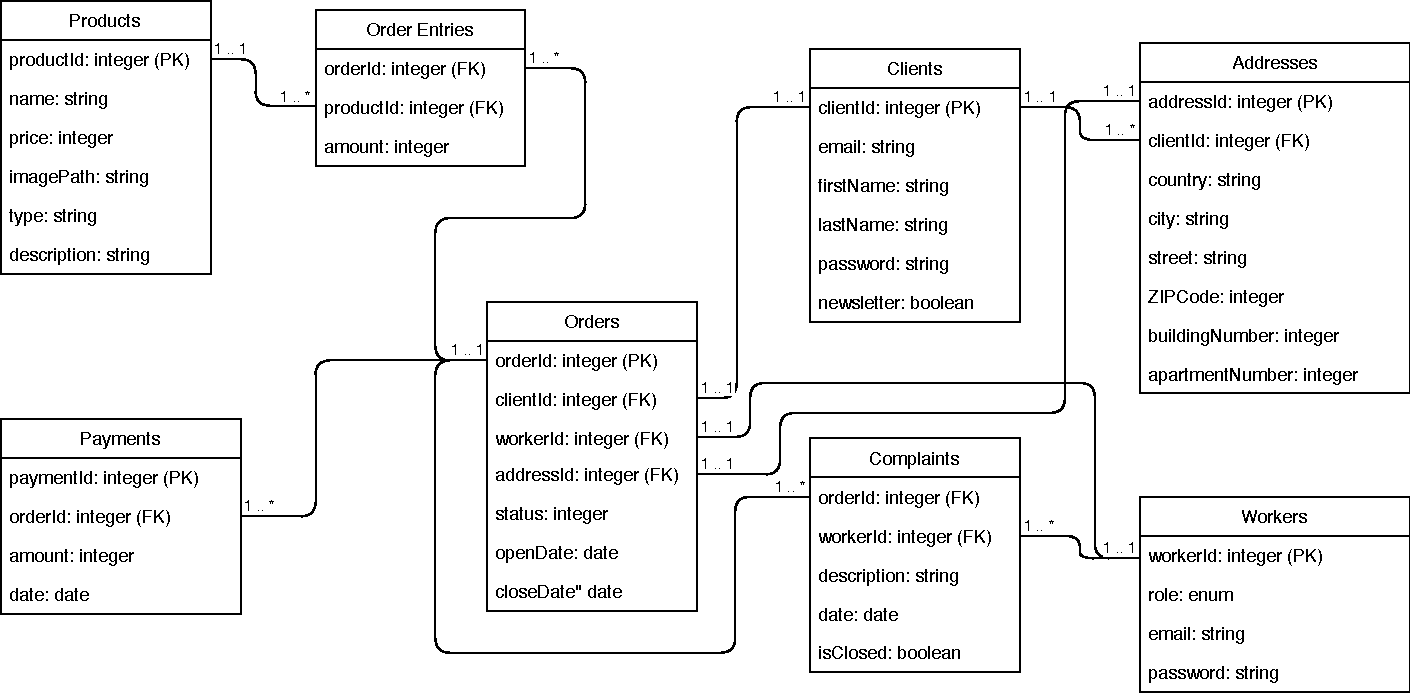
\includegraphics[width=500pt]{database.pdf}
	
	
%---------------------------------------	
	\chapter{Model dynamiki - diagramy STD}
	
%---------------------------------------	
	\chapter{Słownik danych}
	
	\subsubsection{E}
\paragraph{email} $=$ <minimum jeden znak> @ <minimum jeden znak> 
\subsubsection{H}
\paragraph{hasło} $=$ minimum 8 znaków w tym wielka litera, mała litera i cyfra 
\subsubsection{I}
\paragraph{imię}  $=$ minimum jeden znak  
\subsubsection{N}
\paragraph{nazwisko} $=$ minimum jeden znak 


%---------------------------------------	
	\chapter{Technologie i narzędzia}	
		\section{Technologie}
		\begin{itemize}
			\item JavaScript
			\item SignalR
			\item React
			\item nUnit
			\item .NET
			\item JestTest
		\end{itemize}
		
		\section{Narzędzia}
		\begin{itemize}
			\item Visual Studio Code
			\item Visual Studio Community
			\item Selenium
			\item Chromium
			\item CircleCI
		\end{itemize}
	
\end{document}